\chapter{Implementation Part I: The Column Store}
\label{chap:column-store}
% Tell how we want to reduce memory and how database technology comes to the rescue
For the first part of this thesis, our goal is to reduce memory footprint such that client memory requirements can be relaxed. Reduced memory usage are also likely to increase performance due to increased data locality and the cost of memory management. Inspired by the challenges with the current solution which we saw in Section \ref{sec:Challenges with the current solution}, we proceed to use techniques from the field of Database Technology to reduce memory footprint and increase data locality.

% Tell why we pick a column store 
We choose to implement a column store. The reason for this is two-fold. First, as we saw in Section \ref{sub:Row Stores Vs Column Stores}, columns are inherently more compressible. Column stores is, hence, better suited to test our hypothesis and reduce memory footprint than a row-store. Second, the cases where \genus~has experienced performance issues are in situations where a column store is better suited than a row store, for instance on lookup index generation and filter operations.

% Tell why we didn't pick a row store
We believe that transactional processing, where a row store is more suited, will not suffer from using a column-store. On create, update, and delete operations, there constraint checks, validation and memory operations that will make the overhead looking up in multiple columns neglible. Last, row stores mighht rely on indexes that are costly to maintain. Column-stores normally do not need such indexes, because operations on entire columns are efficient \cite{Plattner2014-fr}


\section{CompositionValueCollection}
\label{sec:CompositionValueCollection}
% Lineout the challenges
As we saw in Section \ref{Challenges in Genus App Platform}, one of the challenges in \gap~is the \cn{CompositionObjectValueCollection} class that not only holds the data belonging to each object, but also pointers to the data descriptors. Although this class is flexible because it is self-contained, and can be passed among objects to copy values, for most cases, references to the data descriptors does not generally need to be stored per data collection. 

% Conceptually what is done
\begin{figure}
    \centering
    \begin{subfigure}{1.0\textwidth}
        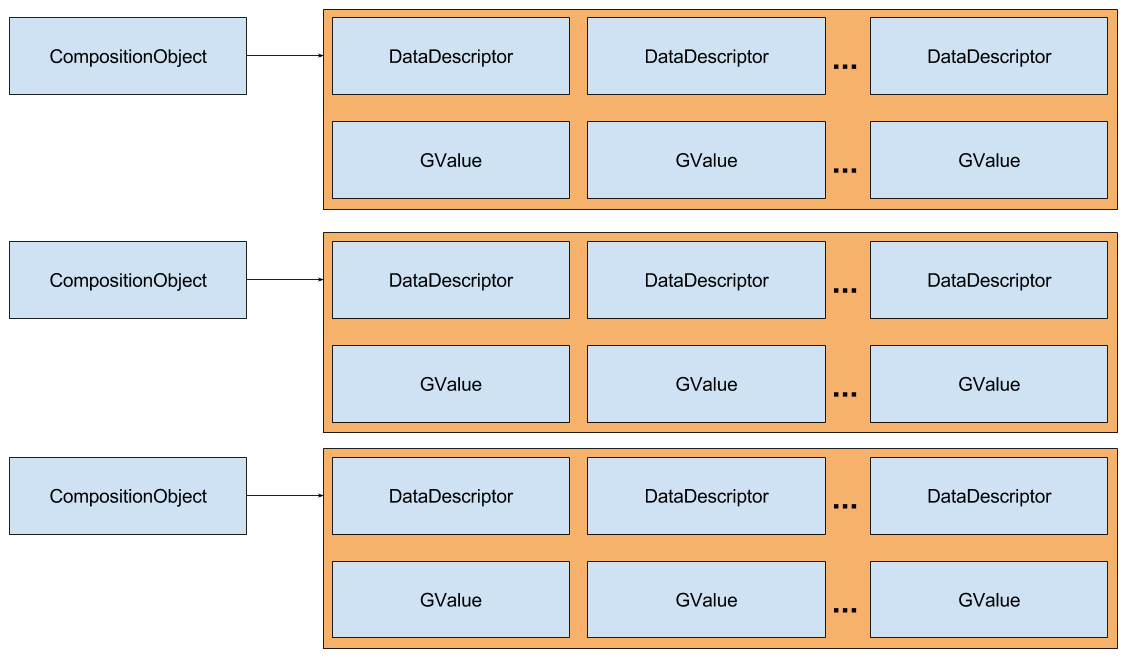
\includegraphics[width=\textwidth]{img/gap-original-rows.png}
        \caption{Original implementation with \cn{CompositionObjectValueColletion}. Each object has its own value collection structure, and each value collection contains pointers to the data descriptors and to the data.}
        \label{fig:gap-original-rows}
    \end{subfigure}
    \begin{subfigure}{1.0\textwidth}
        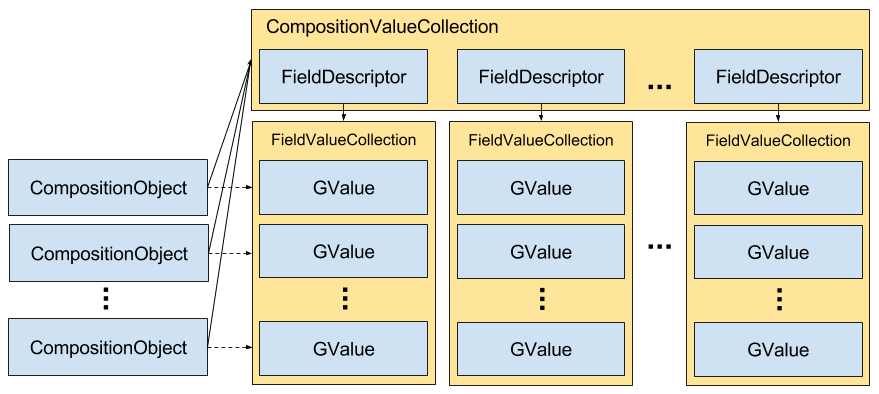
\includegraphics[width=\textwidth]{img/gap-bb-columns.png}
        \caption{Column store implementation with \cn{CompositionValueColletion} and \cn{FieldValueCollection}. All objects in a data source point to the same value collection, and access data using its \cn{DatasourceIndex} which indicates the row number in the columns}
        \label{fig:gap-bb-columns}
    \end{subfigure}
    \caption{Comparison of the original implementation and the column store implementation.}
    \label{fig:gap-storage-comparison}
\end{figure}
In our column store, we plan to replace the \cn{CompositionObjectValueCollection} pointer in each \cn{CompositionObject} with a pointer to a \cn{CompositionValueCollection} and an integer, \cn{DatasourceIndex}, that indicates which position in the data source the object has. All objects within a data source has a pointer to the same \cn{CompositionValueCollection}. This means that composition objects no longer will query its own data collection for values, but rather one common data collection used by all objects. To access a certain value, both \cn{DataDescriptor} and \cn{DatasourceIndex} is required to indicate column and row respectively. A comparison of the old and the new implementation is seen in \ref{fig:gap-storage-comparison}.

% How it impacts memory
In Section \ref{sub:Excessive Amount Of Pointers}, we saw how a data source with objects with 15 properties each needed 32 pointers, or 256 bytes, per objects just for data and data access. Now, this number is reduced to 17 pointers and an integer, which is 140 bytes. Hence, we save 45\% memory by using our new system.

% CompositionObjectValueCollection still exists
Even though the original \cn{CompositionObjectValueCollection} was discarded as the main storage structure, composition objects can still assemble such structures by querying the \cn{CompositionValueCollection}. This is used in object cloning and to transfer data across different data sources in different parts of the application \todo{Stemmer dette?}.

% class diagram
% explain the dictionary and the list of data descriptors
\afigure{img/CompositionValueCollection.png}{\cn{CompositionValueCollection} class diagram.}{fig:CompositionValueCollection}{0.9}
The \cn{CompositionValueCollection} is a class type. The class diagram is shown in Figure \ref{fig:CompositionValueCollection}.

The main methods in the \cn{CompositionValueCollection} class is the \fn{setValue} and \fn{getValue} methods. These functions respectivel set and get \cn{GValues} for a data descriptor and a datasource index. In these operations, the correct column, or \cn{FieldValueCollection}, is looked up in a dictionary, and the index is passed along to the column to get or set the value. If no column exist for a data descriptor, it is created. \fn{isAssigned} and \fn{unassignValue} works similarly. We study the unassigned semantic in Section \ref{sub:Unassigned Values}. 

Datasource indexes are assigned by passing composition objects to the  \fn{registerObject} function. A private variable \vn{maxDatasourceIndex} is used to keep track on the maximum index handed out so far. When an object is received, this variable is incremented and the object is assigned that value. In addition to this, a bitmap \fn{assignedIndexes} is kept to bookkeep which indexes has objects connected to them. When \fn{removeObject} is called, the bit for that index is unset in \fn{assignedIndexes}. In addition, all values corresponding to that object are unassigned. Currently, the \fn{assignedIndexes} bitmap is not used to lookup the first available bit, since this triggers a linear search on every insertion. We discuss this further in the chapter conclusion.

In addition to the above methods, a \cn{CompositionValueCollection} has the ability to unassign an entire row or column by passing in a \cn{CompositionObject} or \cn{DataDescriptor} respectively. We see later in this research where such methods are used.

The \fn{Consolidate} function is called by the data source when it is done loading, and is meant to be an operation where the column store restructures and maximizes space utilization. We see how the columns are affected by this operation in the section about growth strategy, Section \ref{sec:Growth Strategy}.


\section{FieldValueCollection}
\label{sec:FieldValueCollection}
\afigure{img/FieldValueCollection.png}{\cn{FieldValueCollection} class diagram.}{fig:FieldValueCollection}{0.9}
A column is implemented as a \cn{FieldValueCollection} class, and is an index based list structure that automatically handles reallocation. \cn{GValue}s are stored in a \cn{TArray<GValue>}. This array structure was picked based on the performance benchmark in Appndix \ref{app:array-types}. A class diagram for the \cn{FieldValueCollection} is found in Figure \ref{fig:FieldValueCollection}.

Setting a value to \vn{null} has different semantics than \fn{UnassignValue}. The latter means that there has previously been a value present, but is now removed for performance reasons. This functionality is implemented using a bitmap, \cn{BasicBitArray}, which is based on \delphi~\cn{TBits} type. \todo{Stemmer dette om Unassigned values?}

\subsection{Growth Strategy}
\label{sub:Growth Strategy}
Since we used native dynamic arrays, we control the array allocation size. For every reallocation, we risk that the entire array needs to be copied from one part of the memory to another. For this reason, one should be generous when allocating, ideally allocate the correct size immediately. However, since we read a stream of data objects, we are not sure how large our buffers should until the very end. 

\afigure{img/gap-growth-strategy.png}{Growth strategy for buffers. In the load phase, the buffer doubles every time more space is needed. After the load phase, a consolidation is performed which reduces the buffer size to the exact number which are contained in a column.}{fig:gap-growth-strategy}{0.6}
Therefore, we chose a strategy where we double the buffer size every time we need more space. This way, the number of reallocation operations are kept at a minimum. However, this strategy might result in lots of unused buffer space. We, therefore, add a \fn{Consolidate} function to our column store that resizes all buffers to fit its data. The strategy is depicted in \ref{gap-growth-strategy}.

\section{Modifiying CompositionObject}
\label{sec:Modifiying CompositionObject}
% Change value collections and add index
In order for the \cn{CompositionObject} class, some some adjustments are made. First and foremost, the \cn{CompositionObjectValueCollection} are replaced with a \cn{CompositionValueCollection} class. All code that access the original structure are rewritten to use the column store, where the datasource index is passed as a parameter. The \cn{CompositionValueCollection} is already created by the datasource, and is sent in as a parameter in the constructor. It must no longer ask its value collection, it must send itself and its datasource index into the GetValue. It no longer holds ownership to a collection, it has a pointer to a value collection shared by all composition objects.

% Constructor and destructor calls
Second, \fn{RegisterObject} is called within the constructor such that the \cn{CompositionObject} get a datasource index. Analogously, \fn{RemoveObject} is called in the destructor.

% Adapt to the existing value collections with adapts and clone
The class is extended by creating a \fn{CloneValueCollection} that creates a row in the original format. Similarly, a method \fn{AdoptValueCollection} is created to fill inn data from a row structure.

\section{Test results}
\label{sec:Test results}
In this section we test our implementation using Benchmark \ref{bm:q1}, the \textit{TPC-H Q1 Data Load Benchmark}, and Benchmark \ref{bm:write}, the \textit{Write Benchmark}. The first one is run mainly to check whether memory footprint has been reduced, and the second one to see if write performance has been affected by the column store. Full benchmark details are found in Appendix \ref{app:Benchmarks}.

\subsection{TPC-H Result}
\label{sub:TPC-H Result}
Benchmark \ref{bm:q1}, \textit{TPC-H Q1 Data Load Benchmark}, was run with the original and the new column-store implementation with scaling factors 0.01 and 0.1. Each configuration was run three times, and the average of the runs is reported. Only three tests were run due to time constraints. However, all results was within 15 \% of the average value.

\begin{table}
    \centering
    \begin{tabularx}{0.75\textwidth}{X | X X}
        & SF0.01 & SF0.1 \\ 
        \hline
        \hline
        Original & 674 bytes & 715 bytes \\
        Column Store & 419 bytes & 501 bytes \\
        \% reduction & 38 \% & 30 \% \\
    \end{tabularx}
    \caption{Bytes per \texttt{LINEITEM} used by the original and the new column store implementation.} 
    \label{tab:non-blackbox-bpl}
\end{table}
We found a drastic memory reduction with the column store implementation. As seen in Table \ref{tab:non-blackbox-bpl}, the SF0.01 test reduces the memory per \texttt{LINEITEM} by 38 \%, and SF0.1 reduces it by 30 \%. For SF0.1, we also used the total memory footprint output. Total application memory consumption was reduced from 2685 MB to 1777 MB, which is a reduction of 34 \%.

\begin{table}
    \centering
    \begin{tabularx}{0.75\textwidth}{X | X X}
        & SF0.01 & SF0.1 \\ 
        \hline
        \hline
        Original & 2302 ms & 23164 ms \\
        Column Store & 842 ms & 8539 ms \\
        \% reduction & 63 \% & 63 \% \\
    \end{tabularx}
    \caption{Load times for Benchamrk \ref{bm:q1} for the original and the new column store implementation and scaling factors 0.01 and 0.1.} 
    \label{tab:non-blackbox-load}
\end{table}
We see that the load times also is drastically reduced using \cn{CompositionValueCollection}. For both scaling factors, the time it takes to load the datasource with object has been reduced by 63 \%. The results are presented in Table \ref{tab:non-blackbox-load}.

\begin{table}
    \centering
    \begin{tabularx}{0.9\textwidth}{X | X X X}
        SF0.01 & \texttt{LINESTATUS} & \texttt{RETURNFLAG} & \texttt{SHIPDATE}\\ 
        \hline
        \hline
        Original & 300 ms & 313 ms & 1385 ms \\
        Column Store & 391 ms & 401 ms & 1398 ms \\
    \end{tabularx}
    \newline
    \vspace*{1 cm}
    \newline
    \begin{tabularx}{0.9\textwidth}{X | X X X}
        SF0.1 & \texttt{LINESTATUS} & \texttt{RETURNFLAG} & \texttt{SHIPDATE}\\ 
        \hline
        \hline
        Original & 2939 ms & 2849 ms & 13144 ms \\
        Column Store & 3123 ms & 3301 ms & 13004 ms \\
    \end{tabularx}
    \caption{Lookup index generation performance comparison for \texttt{LINESTATUS}, \texttt{RETURNFLAG}, and \texttt{SHIPDATE} for SF0.01 (upper) and SF0.1 (lower).} 
    \label{tab:non-blackbox-lig}
\end{table}
As seen in Table \ref{tab:non-blackbox-lig}, the lookup index generation, or join operation, is hurt by the \cn{CompositionValueCollection} implementation. For scaling factor 0.01, the time it takes to join \texttt{LINESTATUS} and \texttt{RETURNFLAG} with the \texttt{LINEITEM} table is increased by approximately 30 \%.


\begin{table}
    \centering
    \begin{tabularx}{\textwidth}{X | X X X X}
        SF0.01 & \texttt{QUANTITY} & \texttt{EXTENDEDPRICE} & \texttt{DISCOUNT} & \texttt{TAX}\\ 
        \hline
        \hline
        Original & 30 ms & 34 ms & 32 ms & 35 ms \\
        Column Store & 57 ms & 67 ms & 75 ms & 76 ms
    \end{tabularx}
    \newline
    \vspace*{1 cm}
    \newline
    \begin{tabularx}{\textwidth}{X | X X X X}
        SF0.01 & \texttt{QUANTITY} & \texttt{EXTENDEDPRICE} & \texttt{DISCOUNT} & \texttt{TAX}\\ 
        \hline
        \hline
        Original & 302 ms & 385 ms & 312 ms & 369 ms \\
        Column Store & 532 ms & 625 ms & 646 ms & 752 ms
    \end{tabularx}
    \caption{Source measure lookup for \texttt{QUANTITY} \texttt{EXTENDEDPRICE}, \texttt{DISCOUNT}, and \texttt{TAX} for SF0.01 (upper) and SF0.1 (lower).} 
    \label{tab:non-blackbox-sml}
\end{table}
We also see that source measure looukup is also hurt by the new column store implementation, where the the time it takes to extract all values into a floating point array is doubled. The results are presented in Table \ref{tab:non-blackbox-sml}.

\subsection{Write Benchmark}
\label{sub:Write Benchmark}
In order to see how the write speed is affected by our new implementation, we run Benchmark \ref{bm:write}, the \textit{Write Benchmark} on the original implementation and on the column store implementation. Each run modified 1000 elements. Due to time constraints, there were only three runs per implementation. However, most measurements was within 15 \% of the average.

\begin{table}
    \begin{tabularx}{\textwidth}{X | X X X X}
         & \texttt{QUANTITY} & \texttt{EXTENDEDPRICE} & \texttt{COMMENT} & \texttt{SHIPDATE}\\ 
        \hline
        \hline
        Original & 1657 ms & 1675 ms & 1669 ms & 2060 ms \\
        Column Store & 1642 ms & 1610 ms & 1770 ms & 2046 ms
    \end{tabularx}
    \caption{Test results for Benchmark \ref{bm:write}.}
    \label{tab:non-blackbox-write}
\end{table}
The results are presented in Table \ref{tab:non-blackbox-write}. There are not more differences between the two implementations that are expected by random, except for \texttt{COMMENT}. This result had an outlier.

\section{Discussion}
\label{sec:Discussion}
We conclude that our hypothesis is right, pointers take up a lot of space. By doing no other changes but removing the data descriptor pointers for all objects, the memory used per object is reduced by 38 \% and 30 \% respectively for scaling factors 0.01 and 0.1 respectively. 

We are excited to see that data source load time has been drastically reduced. We are unsure why the load times have been reduced by as much as 63 \%, but this might strengthen the proof on the hypothesis that memory management is expensive. Due to our growth strategy, the number of allocations are drastically reduced. The original implementation allocated one \cn{CompositionObjectValueCollection} for each object. The new implementation only double all column capacity 20 times during a data load. Secondly, if the process is memory bound, reduced memory usage correlates directly with improved performance. Finally, our new implementation might have improved memory locality and cache hit rate. 

Both lookup index creating and source measure lookup operations suffer from the new implementation, where the time it takes to perform the operation has been increased by roughly 30 \% and 100 \% respectively. Both operations read values intensively from the columns, so it is likely that \fn{GetValue} in \cn{CompositionValueCollection} as it is in \cn{CompositionObjectValueCollection}. This can be caused by the dictionary lookup to find the correct column, or extra checks to ensure capacity or for \vn{null} values.

Benchmark \ref{bm:write} yielded equal results for both implementations, even though most operations in Benchmark \ref{bm:q1} were slowed down by the column store. However, put in perspective, the operations from the \textit{TPC-H Q1 Load Benchmark} use almost as long time on 600,000 elements that \textit{Write Benchmark} uses on 1,000 elements. This indicates that there is a severe overhead in object iteration and value modification that is unrelated to how the data storage layout.

We are unsure why there is a different space saving for different scaling factors. However, for the other measures, scaling factors seem to scale as they should. It might be caused by the caching and value reuse in load mechanisms in \gap, and that different data size is affected by the total number of rows. The data might also be skewed, which means SF0.01 has more values that can be reused. Either way, we see that both original and column store presentation is affected similarly, which means that the effect is unrelated to our work.

\section{Chapter Conclusion}
\label{sec:Chapter Conclusion}
We conclude that there is a large potential in column storage in terms of memory footprint, and that load time is reduced with our new column store implementation. In total, the \gd~application that loads the \tpch~ with a scaling factor of 0.1 have reduced memory usage from 2685 MB to 1777 MB, and the load time is reduced by more than half.

Still, most operations in our benchmarks perform worse using the \cn{CompositionValueCollection} class. Especially the source measure lookup operation, which shows that generating an array of double precision floating point values takes twice as long using our new column store implementation.

We believe even more memory can be saved, and load time improved, by optimizing storage formats, applying compression, and removing more pointers. We do this in Chapter \ref{chap:part2}. We are also confident that the join and source measure lookup operations can be rewritten to exploit the new storage format. We look into this in Chapter \ref{chap:part3}.

\subsection{Future Work}
\label{sub:Future Work}
Now, we only assign new datasource indexes by incrementing, however we have put in a bitmap for assigned flags. We have disregarded this structure due to the linear search to find the first open bit, and that neither of our benchmarks inserts and removes certain objects. Future work might investigate the effects of using \fn{OpenBit}, and perhaps separate between loading and normal state. The \fn{Consolidate} function might also be used to compress the data and make sure all columns are used.

In addition, we have observed that the bytes per \texttt{LINEITEM} is increased on larger data sets, and we believe this is caused by the caching and value reuse mechanisms in the data source loader. However, larger datasets should be able to reuse more values, not less. We therefore encourage studying this peculiar effect in future work.
